\documentclass[aspectratio=43]{beamer}
\usepackage[utf8]{inputenc}
\usepackage[T1]{fontenc}
\usepackage{graphicx}
\usepackage{booktabs}
\usepackage{tabularx}
\usepackage{array}
\usepackage{tikz}
\usetikzlibrary{positioning,arrows.meta}
\usepackage{pgfplots}
\usepackage{hyperref}
\usepackage{listings}
\usepackage{xcolor}
\pgfplotsset{compat=1.18}

\usetheme{Madrid}
\usecolortheme{default}
\setbeamertemplate{navigation symbols}{}
\setbeamertemplate{caption}[numbered]
\setbeamercolor{structure}{fg=blue!55!black}
\setbeamercolor{block title}{fg=white,bg=blue!60!black}
\setbeamercolor{block body}{bg=blue!4}
\setbeamercolor{alertblock title}{fg=white,bg=red!65!black}
\setbeamercolor{alertblock body}{bg=red!4}
\lstset{
  language=Python,
  basicstyle=\ttfamily\scriptsize,
  keywordstyle=\color{blue!60!black},
  commentstyle=\color{black!55},
  stringstyle=\color{red!55!black},
  showstringspaces=false,
  breaklines=true,
  frame=single,
  rulecolor=\color{blue!25},
  numbers=none,
  xleftmargin=0.15cm,
  xrightmargin=0.15cm,
  aboveskip=0.12cm,
  belowskip=0.12cm
}

\graphicspath{{./}{../generated/}}

\title[Agent-Based Crowd Simulation]
{Integrating Computer Vision: Agent-Based Crowd Simulation for Stampede Prevention and Event Safety}
\subtitle{Project Review}
\author[Group 4]{\textbf{Project Team:}\\
Nivin P Louis (TL23BTAI0042)\\
Niranjana Sreevalsan (TL23BTAI0348)\\
Farhan Mohamed T P (TL23BTAI0308)\\
Nihal P Shakeer (TL23BTAI0249)\\[0.20cm]
\textbf{Project Guide:}\\Anju K P, Assistant Professor, Dept. AIML}
\institute[Dept. AIML]{Vidya Academy of Science and Technology, Thrissur}
\date[October 4, 2026]{}

\newcommand{\smallnote}[1]{{\tiny\color{black!65}#1}}

\begin{document}

% 1
\frame{\titlepage}

% 2
\begin{frame}
\centering

\includegraphics[width=0.10\textwidth]{college_logo.png}\\[0.5mm]
{\small\bfseries College Vision}\\[0.4mm]
{\fontsize{7}{7.3}\selectfont To be a premier institution in engineering education and research, nurturing innovative professionals for sustainable societal development.}\\[0.5mm]
{\small\bfseries College Mission}\\[0.4mm]
\begin{minipage}{0.99\textwidth}\fontsize{7}{7.3}\selectfont
\raggedright
\textbf{M1:} Provide quality engineering education that empowers students with strong technical competence and analytical problem solving abilities.\par
\textbf{M2:} Promote research, innovation, entrepreneurship and industry collaboration to develop sustainable technological solutions.\par
\textbf{M3:} Develop ethical and socially responsible professionals with leadership qualities, lifelong learning abilities and a commitment to societal well-being.
\end{minipage}\\[0.7mm]
{\small\bfseries Department Vision}\\[0.4mm]
{\fontsize{7}{7.3}\selectfont To be a center of excellence in artificial intelligence and machine learning education, research, and innovation, nurturing competent professionals capable of developing intelligent, ethical, and sustainable solutions for societal and industrial advancement.}\\[0.5mm]
{\small\bfseries Department Mission}\\[0.4mm]
\begin{minipage}{0.99\textwidth}\fontsize{7}{7.3}\selectfont
\raggedright
\textbf{M1:} Provide quality education in artificial intelligence and machine learning through effective teaching-learning practices, enabling students to acquire strong technical knowledge, analytical skills, and problem-solving abilities.\par
\textbf{M2:} Promote research, innovation, entrepreneurship, and interdisciplinary collaboration in emerging AI technologies to address industrial and societal challenges.\par
\textbf{M3:} Develop professionally competent graduates with ethical values, leadership qualities, lifelong learning abilities, and a commitment to societal well-being in a technology-driven world.
\end{minipage}
\end{frame}

% 3
\begin{frame}\frametitle{Index}\tableofcontents\end{frame}

% Problem Statement
\section{Problem Statement}
% 4
\begin{frame}\frametitle{Problem Statement}
\large
\begin{block}{Problem Statement}
Public venues generate dynamic pedestrian flows that static counts cannot describe. This project uses observed ATC trajectories and a ROS floor map to replay and simulate pedestrian movement, then checks short-horizon forecasts against held-out tracks.
\end{block}
\vspace{0.12cm}
\begin{itemize}
\setlength\itemsep{0.18cm}
\item Counts and fixed capacity do not show individual routes or how movement changes over time.
\item Real trajectories ground the simulator in observed speeds, paths, and starting states.
\item Map-constrained agents provide a repeatable way to explore movement scenarios and compare forecasts.
\end{itemize}
\end{frame}

% 1 Motivation
\section{Motivation}
% 5
\begin{frame}\frametitle{Motivation}
\large
\begin{itemize}
\setlength\itemsep{0.22cm}
\item Observed pedestrian trajectories ground the simulator in measured paths and speeds.
\item Individual agents make route and movement assumptions explicit.
\item A mapped environment shows how pedestrian paths and density evolve over time.
\item Replay and held-out comparisons let us inspect how simulation tracks observed movement.
\item Repeatable simulation supports future study of event-safety scenarios under stated assumptions.
\end{itemize}
\end{frame}

% 2 Objectives
\section{Objectives}
% 6
\begin{frame}\frametitle{Objectives}
\large
\begin{itemize}
\setlength\itemsep{0.16cm}
\item \textbf{Prepare trajectories:} Clean ATC records, convert units, and summarize speed, routes, and endpoint zones.
\item \textbf{Align the environment:} Use the ROS occupancy map to constrain simulated movement to walkable cells.
\item \textbf{Initialize agents:} Start from observed snapshots or empirical movement profiles.
\item \textbf{Simulate pedestrian flow:} Advance Social Force agents with map-based routing and obstacle rejection.
\item \textbf{Evaluate forecasts:} Compare 1-, 5-, and 10-second predictions with held-out tracks and a constant-velocity baseline.
\item \textbf{Visualize movement:} Inspect observed tracks, simulated flow, and forecast summaries in the replay dashboard.
\end{itemize}
\end{frame}

% 3 Literature Review
\section{Literature Review}
% 6
\begin{frame}\frametitle{Literature Review}
\small
\begin{itemize}
\item \textbf{Microscopic crowd models:} agent-based studies represent individual traits, goals, and interactions [3].
\item \textbf{Observation-informed simulation:} research has combined crowd observations with agent-based models to forecast movement [4].
\item \textbf{Evacuation and layout studies:} compare routes, exits, and scenarios using simulated agents [5].
\item \textbf{Computer-vision studies:} estimate people, density, or flow from images, but require reliable camera-to-floor calibration for spatial simulation.
\end{itemize}
\vspace{0.16cm}
\begin{block}{Literature takeaway}
The supplied review spans computer vision, agent-based movement, and evacuation planning. The present implementation focuses on connecting real pedestrian trajectories to a mapped simulator.
\end{block}
\note{This slide summarizes the supplied literature review. Representative references: Khan and Deng (2024); Makinoshima and Oishi (2022); Alidmat et al. (2025). See References.}
\end{frame}

% 7
\begin{frame}\frametitle{Research Gap and Project Position}
\begin{columns}[T,onlytextwidth]
\column{0.48\textwidth}
\begin{block}{What prior work motivates}
\begin{itemize}
\item Individual movement rules matter for crowd-level outcomes.
\item Real observations can inform simulation state and behaviour.
\item Layout and route changes can be studied through scenarios.
\end{itemize}
\end{block}
\column{0.48\textwidth}
\begin{block}{What this prototype contributes}
\begin{itemize}
\item ATC trajectories aligned to the supplied ROS occupancy map.
\item Empirical route and speed profiles used by Social Force agents.
\item Held-out normal-flow forecast comparison in a replay dashboard.
\end{itemize}
\end{block}
\end{columns}
\end{frame}

% 5 Architecture
\section{Architecture}
% 9
\begin{frame}\frametitle{System Architecture}
\centering
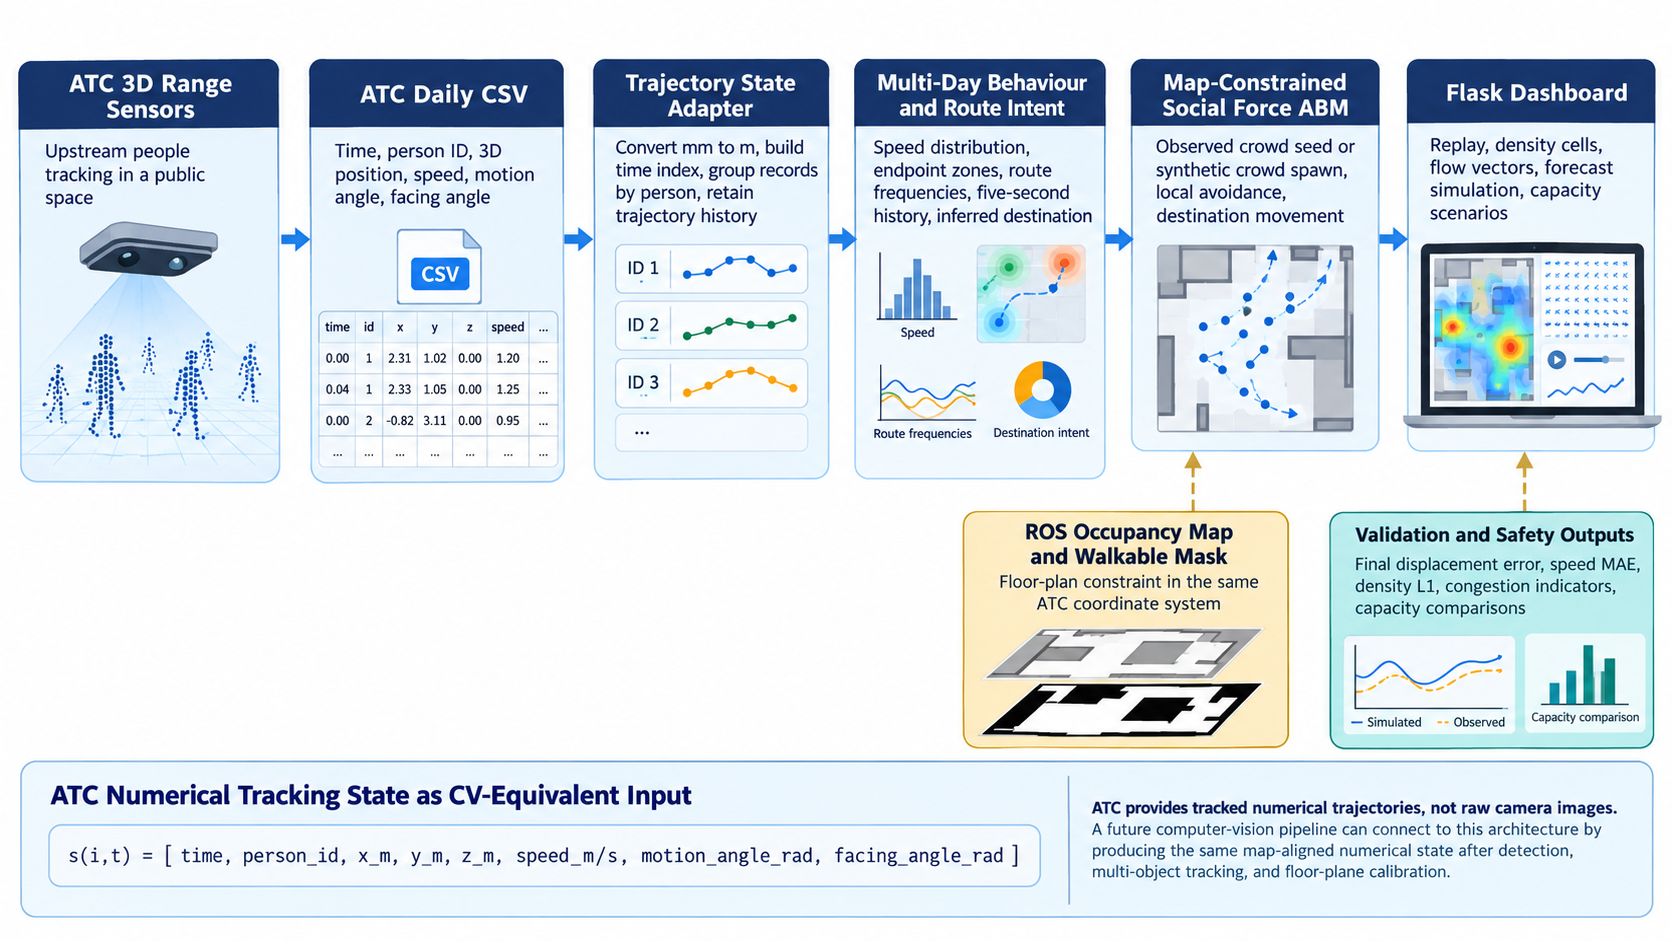
\includegraphics[width=0.98\textwidth,height=0.76\textheight,keepaspectratio]{system_architecture.png}
\end{frame}

% 6 Methodology
\section{Methodology}
% 10
\begin{frame}\frametitle{Data and Environment}
\begin{columns}[T,onlytextwidth]
\column{0.55\textwidth}
\begin{itemize}
\item ATC shopping-centre tracks from a 3D range-sensor system, Osaka, Japan [1, 2].
\item 10 locally available daily files from Oct--Nov 2012.
\item Each observation records time, ID, position, speed, motion angle, and facing angle.
\item Positions use millimetres; speed uses millimetres per second.
\item The ROS occupancy map uses the same coordinate frame [1].
\end{itemize}
\column{0.42\textwidth}
\centering
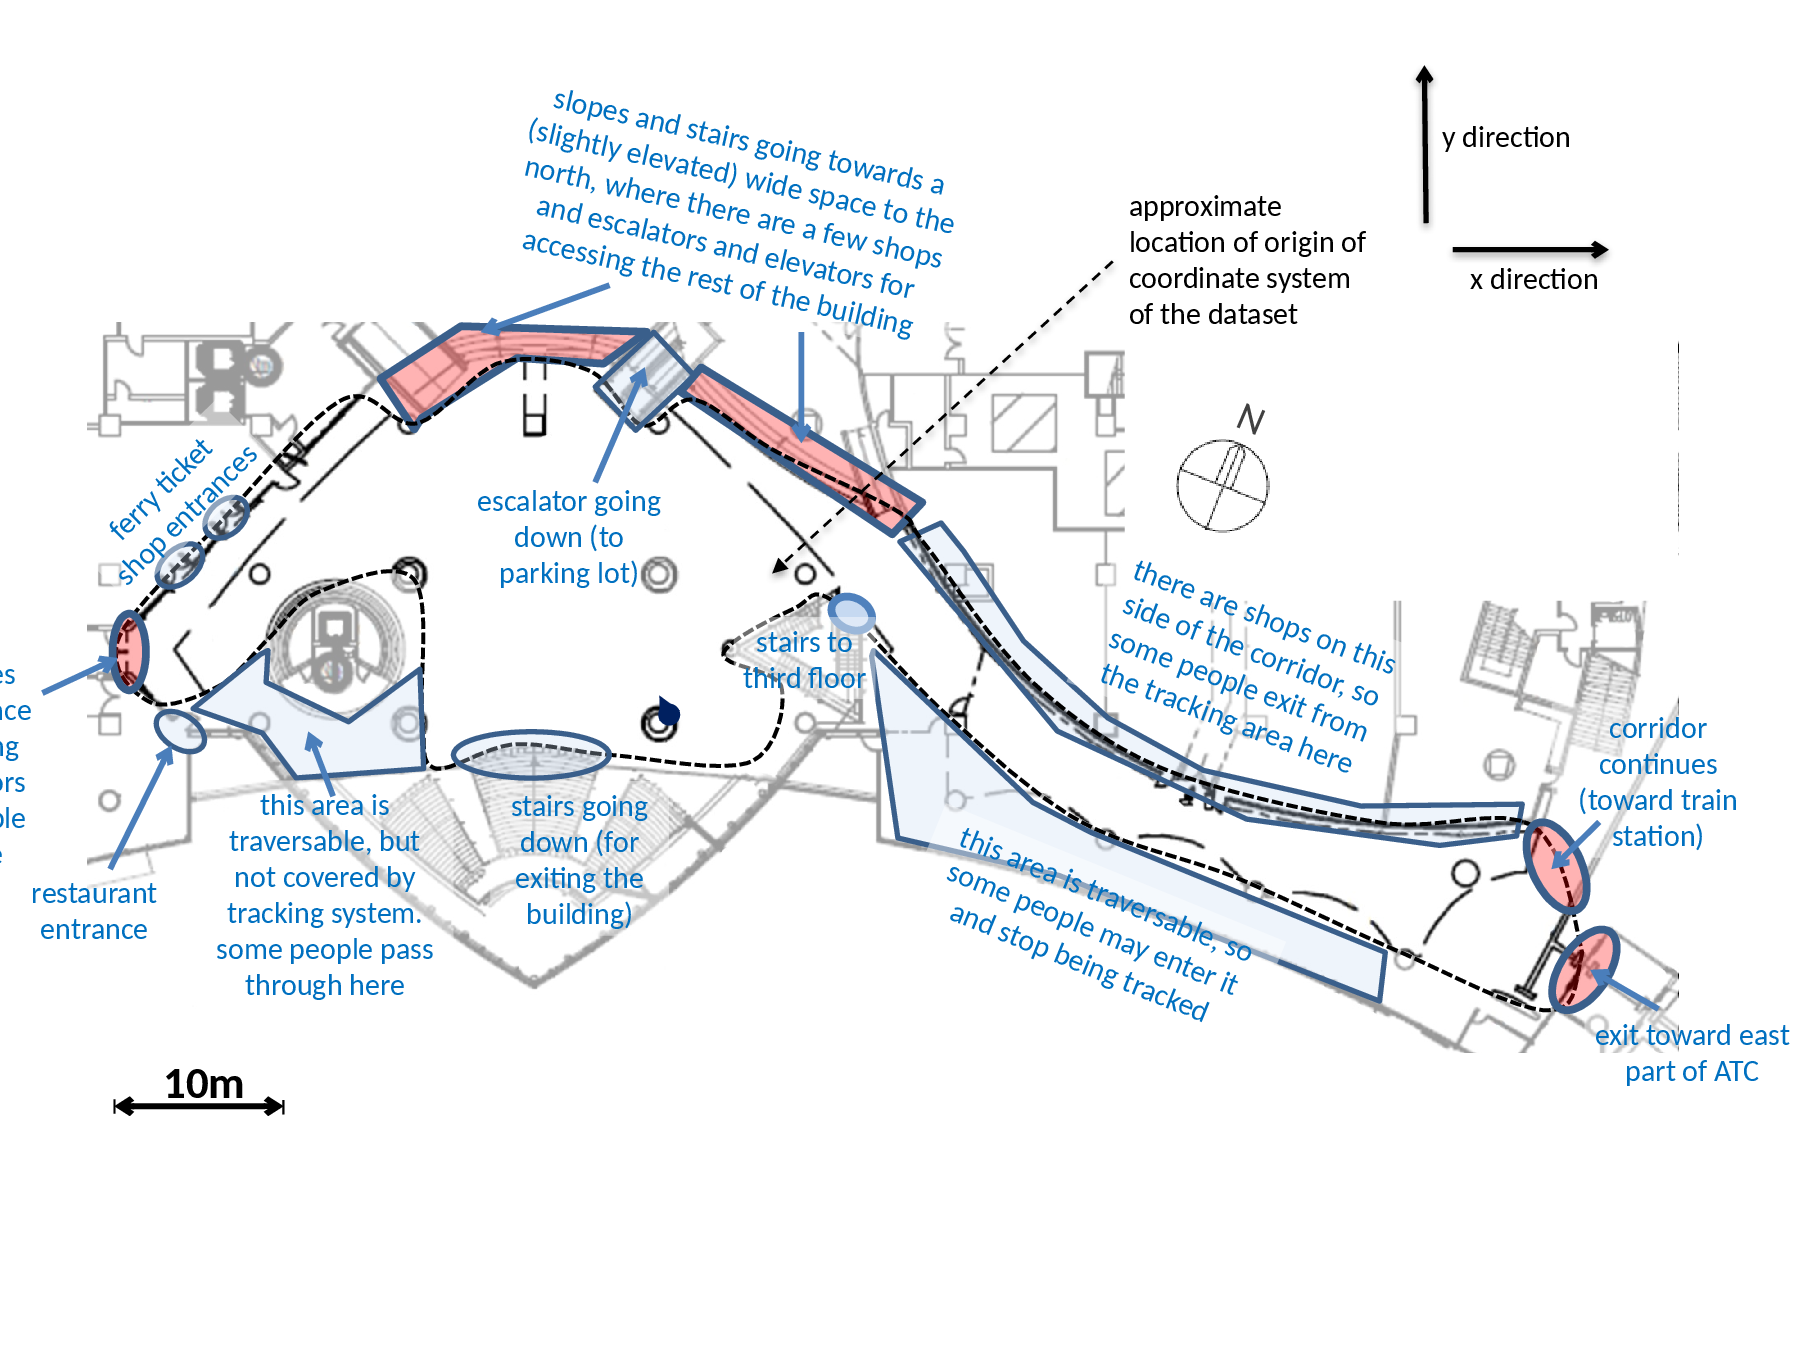
\includegraphics[width=\linewidth]{atc_floorplan.png}\\[-1mm]
\smallnote{Supplied ATC floor-plan slide}
\end{columns}
\end{frame}

% 11
\begin{frame}\frametitle{Data Preparation}
\small
\begin{enumerate}
\item Stream each daily CSV and build minute-level byte-offset indexes for interval replay.
\item Convert position and speed to metres and metres per second.
\item Filter trajectory jumps above 4 m and gaps outside 0.01--1.0 s.
\item Retain trajectories with at least 30 seconds and 20 samples.
\item Aggregate speed, heading, provisional endpoint zones, and frequent routes.
\end{enumerate}
\vspace{0.16cm}
\begin{block}{10-day data profile}
307.7 million observations \hfill 340,953 tracked IDs\\
165,089 filtered trajectories \hfill Mean speed: 0.839 m/s
\end{block}
\smallnote{Endpoint clusters are provisional analysis zones, not confirmed doors.}
\end{frame}

% 12
\begin{frame}\frametitle{Agent-Based Simulation}
\small
Each pedestrian agent stores position, velocity, desired speed, facing direction, radius, destination, and arrival state.
\vspace{0.14cm}
\begin{block}{Movement update}
Agents follow a map-based shortest path toward a sampled destination. Nearby pedestrians contribute a distance-based repulsion, weighted by the agent's facing direction.
\end{block}
The model advances in 0.1 s steps, caps speed at 2.0 m/s, and rejects moves into non-walkable cells.
\vspace{0.12cm}
\begin{itemize}
\item \textbf{Observed start:} initialise agents from a selected crowd snapshot.
\item \textbf{Synthetic start:} sample route, endpoint zone, and speed from empirical profiles.
\end{itemize}
\smallnote{Normal-flow calibration selected near-zero repulsion; dense-flow interaction behaviour remains unvalidated.}
\note{The movement model follows the Social Force family [6] with map-grid route following. The held-out forecast uses the calibrated parameter set.}
\end{frame}

% 13
\begin{frame}\frametitle{Forecast Evaluation}
\small
\begin{enumerate}
\item Calibrate parameters on three 10-second snapshots from 11 Nov 2012.
\item Hold out 14 Nov 2012; exclude that date from the calibration profile.
\item At six test times, seed the model from observations and five seconds of past history.
\item Compare the 1, 5, and 10-second forecasts with later observations for matching IDs.
\item Compare against constant velocity using the same starting observations.
\end{enumerate}
\vspace{0.14cm}
\begin{block}{Metrics}
\textbf{FDE:} mean endpoint distance in metres. \quad
\textbf{Density $L_1$:} difference in people-counts over 2 m cells, normalized by matched people.\\
\textbf{Speed MAE:} mean absolute speed error in m/s.
\end{block}
\end{frame}

% 7 Implementation
\section{Implementation}
% 14
\begin{frame}\frametitle{Dashboard Implementation}
\centering
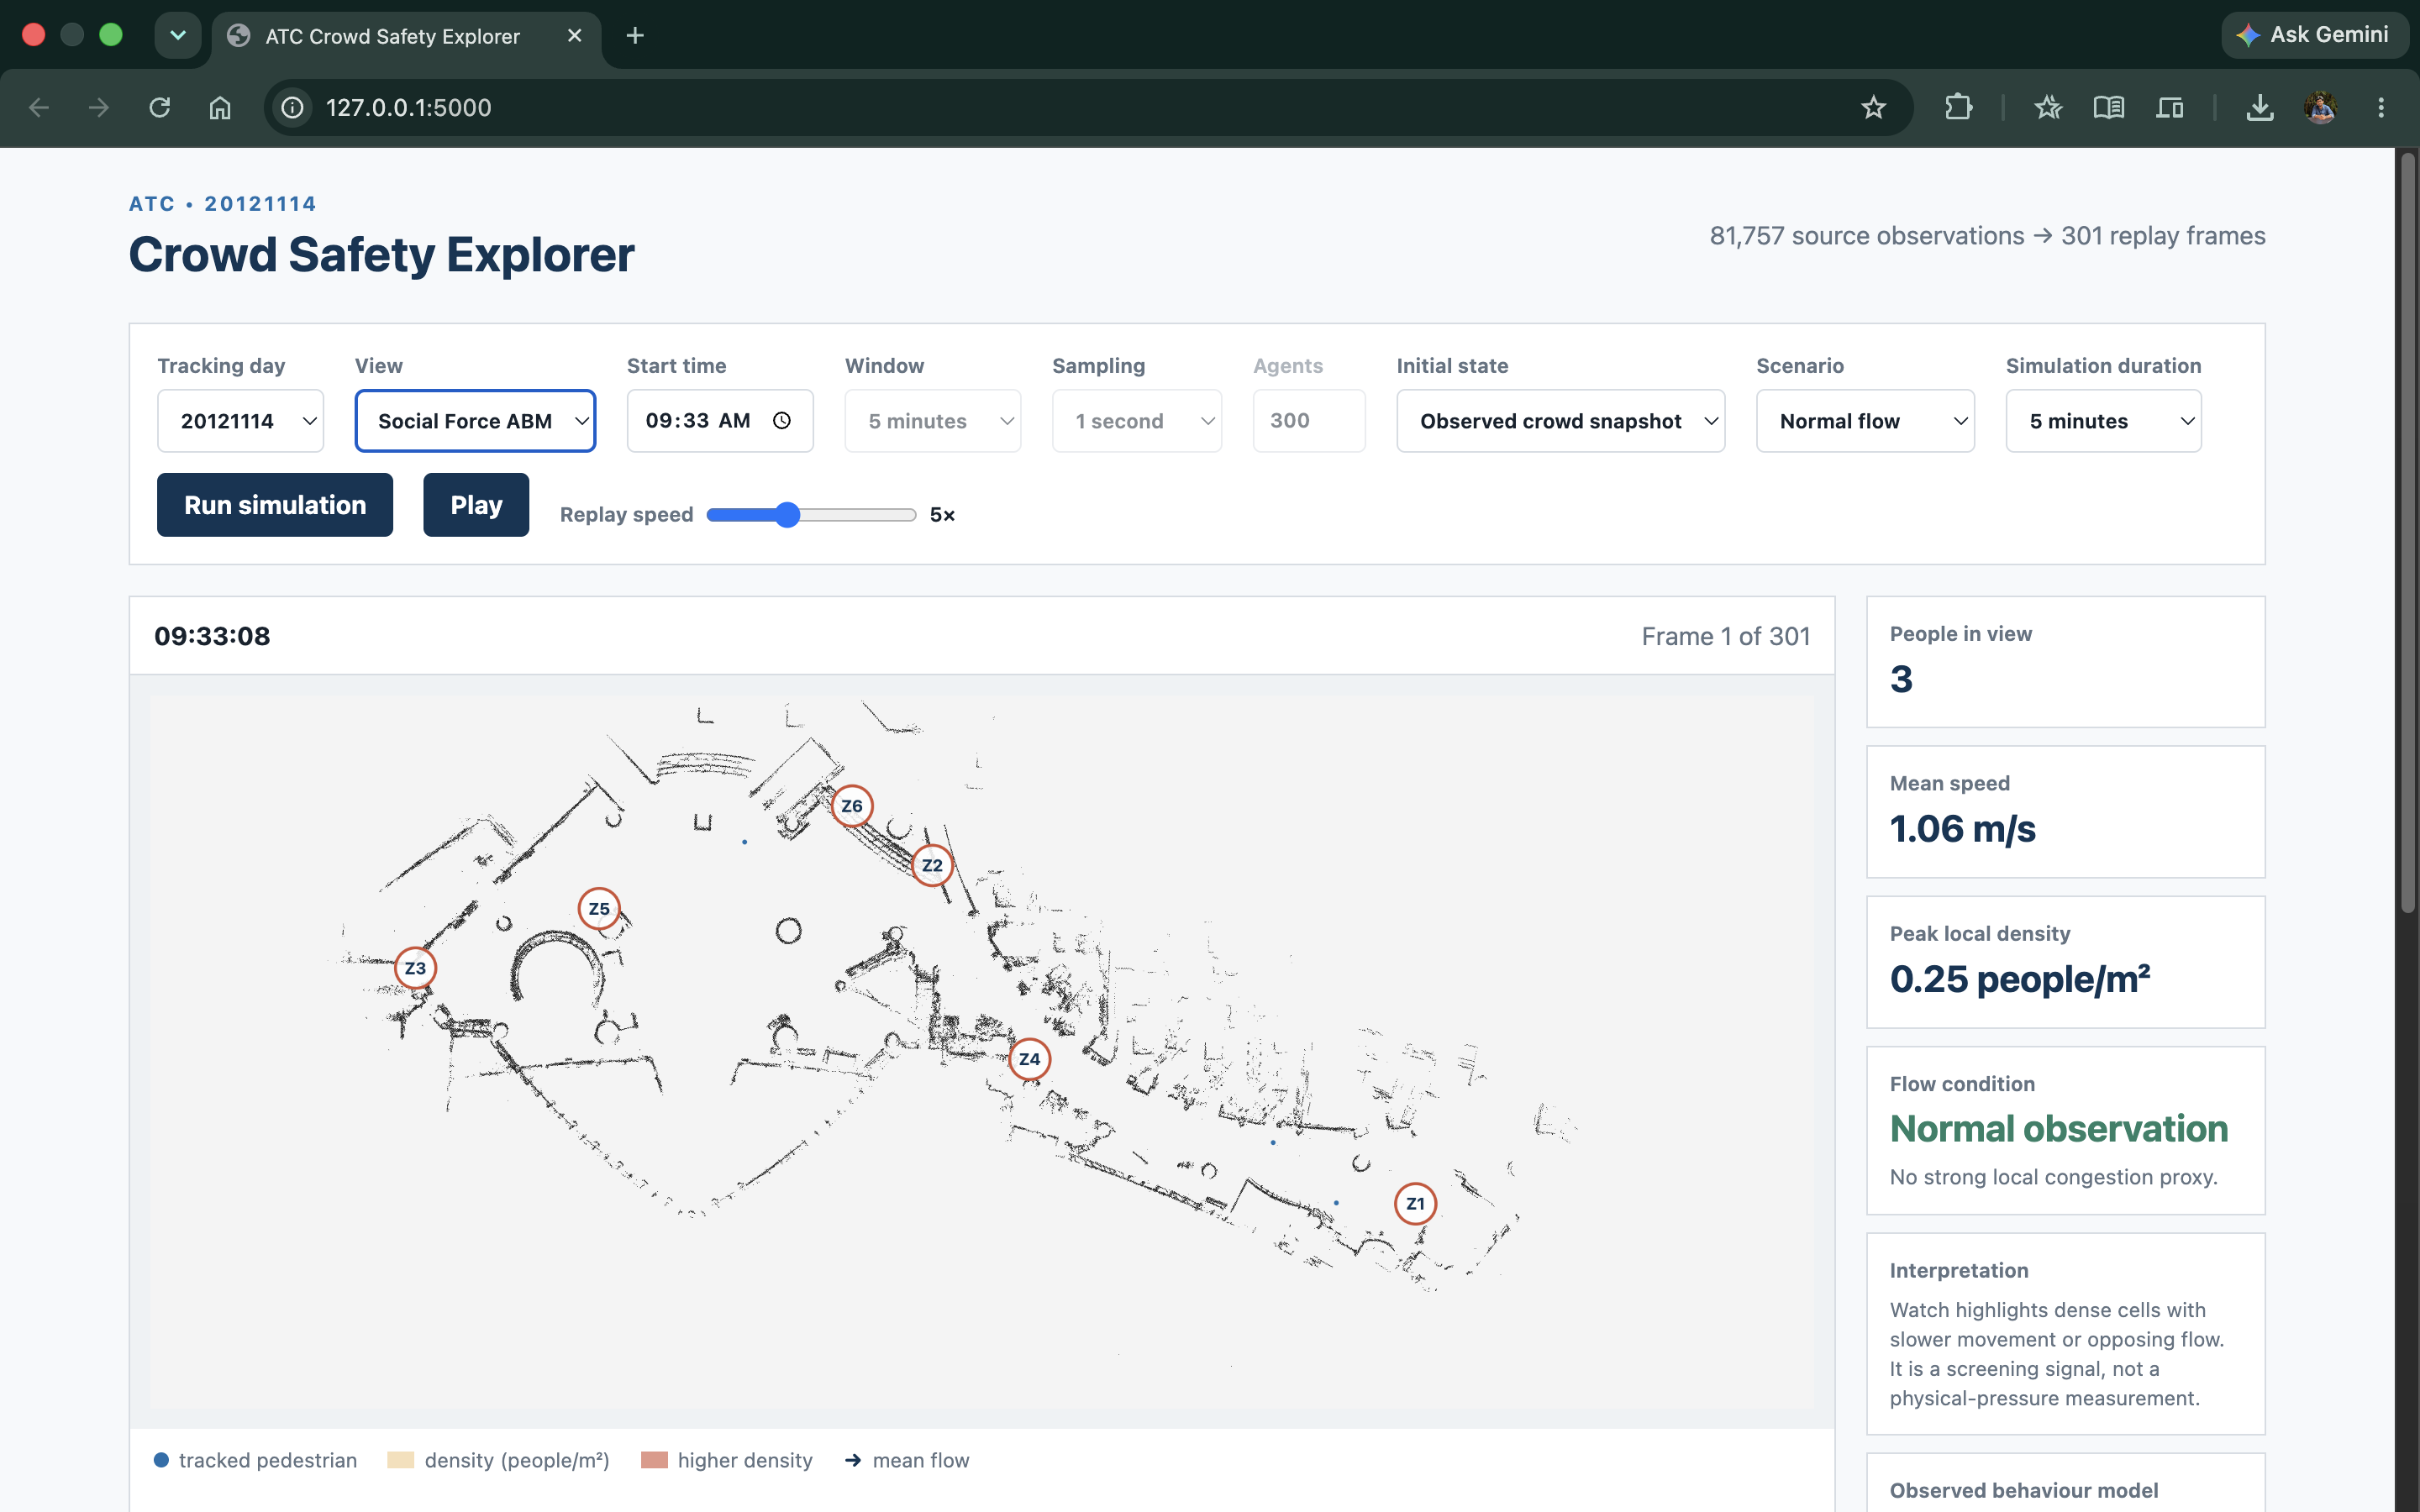
\includegraphics[width=0.99\textwidth,height=0.83\textheight,keepaspectratio]{dashboard_screenshot.png}
\note{Dashboard screenshot showing the map replay view, simulation controls, and crowd metrics.}
\end{frame}

% 15
\begin{frame}\frametitle{Implementation Results}
\centering
\begin{tikzpicture}
\begin{axis}[
  ybar,bar width=14pt,width=0.82\textwidth,height=0.55\textheight,
  ylabel={Mean FDE (m)}, symbolic x coords={1 s,5 s,10 s},xtick=data,
  ymin=0,ymax=5.6,legend style={at={(0.5,-0.18)},anchor=north,legend columns=2},
  nodes near coords, every node near coord/.append style={font=\scriptsize},
  ymajorgrids=true,grid style={black!10},enlarge x limits=0.3]
\addplot[fill=blue!62] coordinates {(1 s,0.377) (5 s,1.567) (10 s,3.505)};
\addplot[fill=orange!75] coordinates {(1 s,0.458) (5 s,2.338) (10 s,4.986)};
\legend{Social Force,Constant velocity}
\end{axis}
\end{tikzpicture}\\[-1mm]
\small
FDE improved by 17.74\%, 33.00\%, and 29.71\% at 1, 5, and 10 seconds.
\smallnote{Six held-out snapshots per horizon on 14 Nov 2012; normal-flow trajectory forecasting only.}
\end{frame}

% 16
\begin{frame}\frametitle{Held-Out Results}
\small
\begin{table}
\centering
\begin{tabularx}{0.94\textwidth}{p{1.25cm} X X p{2.15cm}}
\toprule
Horizon & FDE (SF / CV) & Density $L_1$ (SF / CV) & Speed MAE (SF) \\
\midrule
1 s & 0.377 / 0.458 m & 0.473 / 0.529 & 0.302 m/s \\
5 s & 1.567 / 2.338 m & 1.032 / 1.441 & 0.452 m/s \\
10 s & 3.505 / 4.986 m & 1.364 / 1.805 & 0.565 m/s \\
\bottomrule
\end{tabularx}
\end{table}
\begin{block}{Test coverage}
All six requested snapshots had matched tracks. The 10-second results contain 77 matched person-snapshot pairs.
\end{block}
\smallnote{The experiment does not evaluate panic, physical pressure, stampede detection, or evacuation success.}
\end{frame}

% 8 Code Snippets
\section{Code Snippets}
% 17
\begin{frame}\frametitle{Code Implementation: Track Cleaning}
\centering
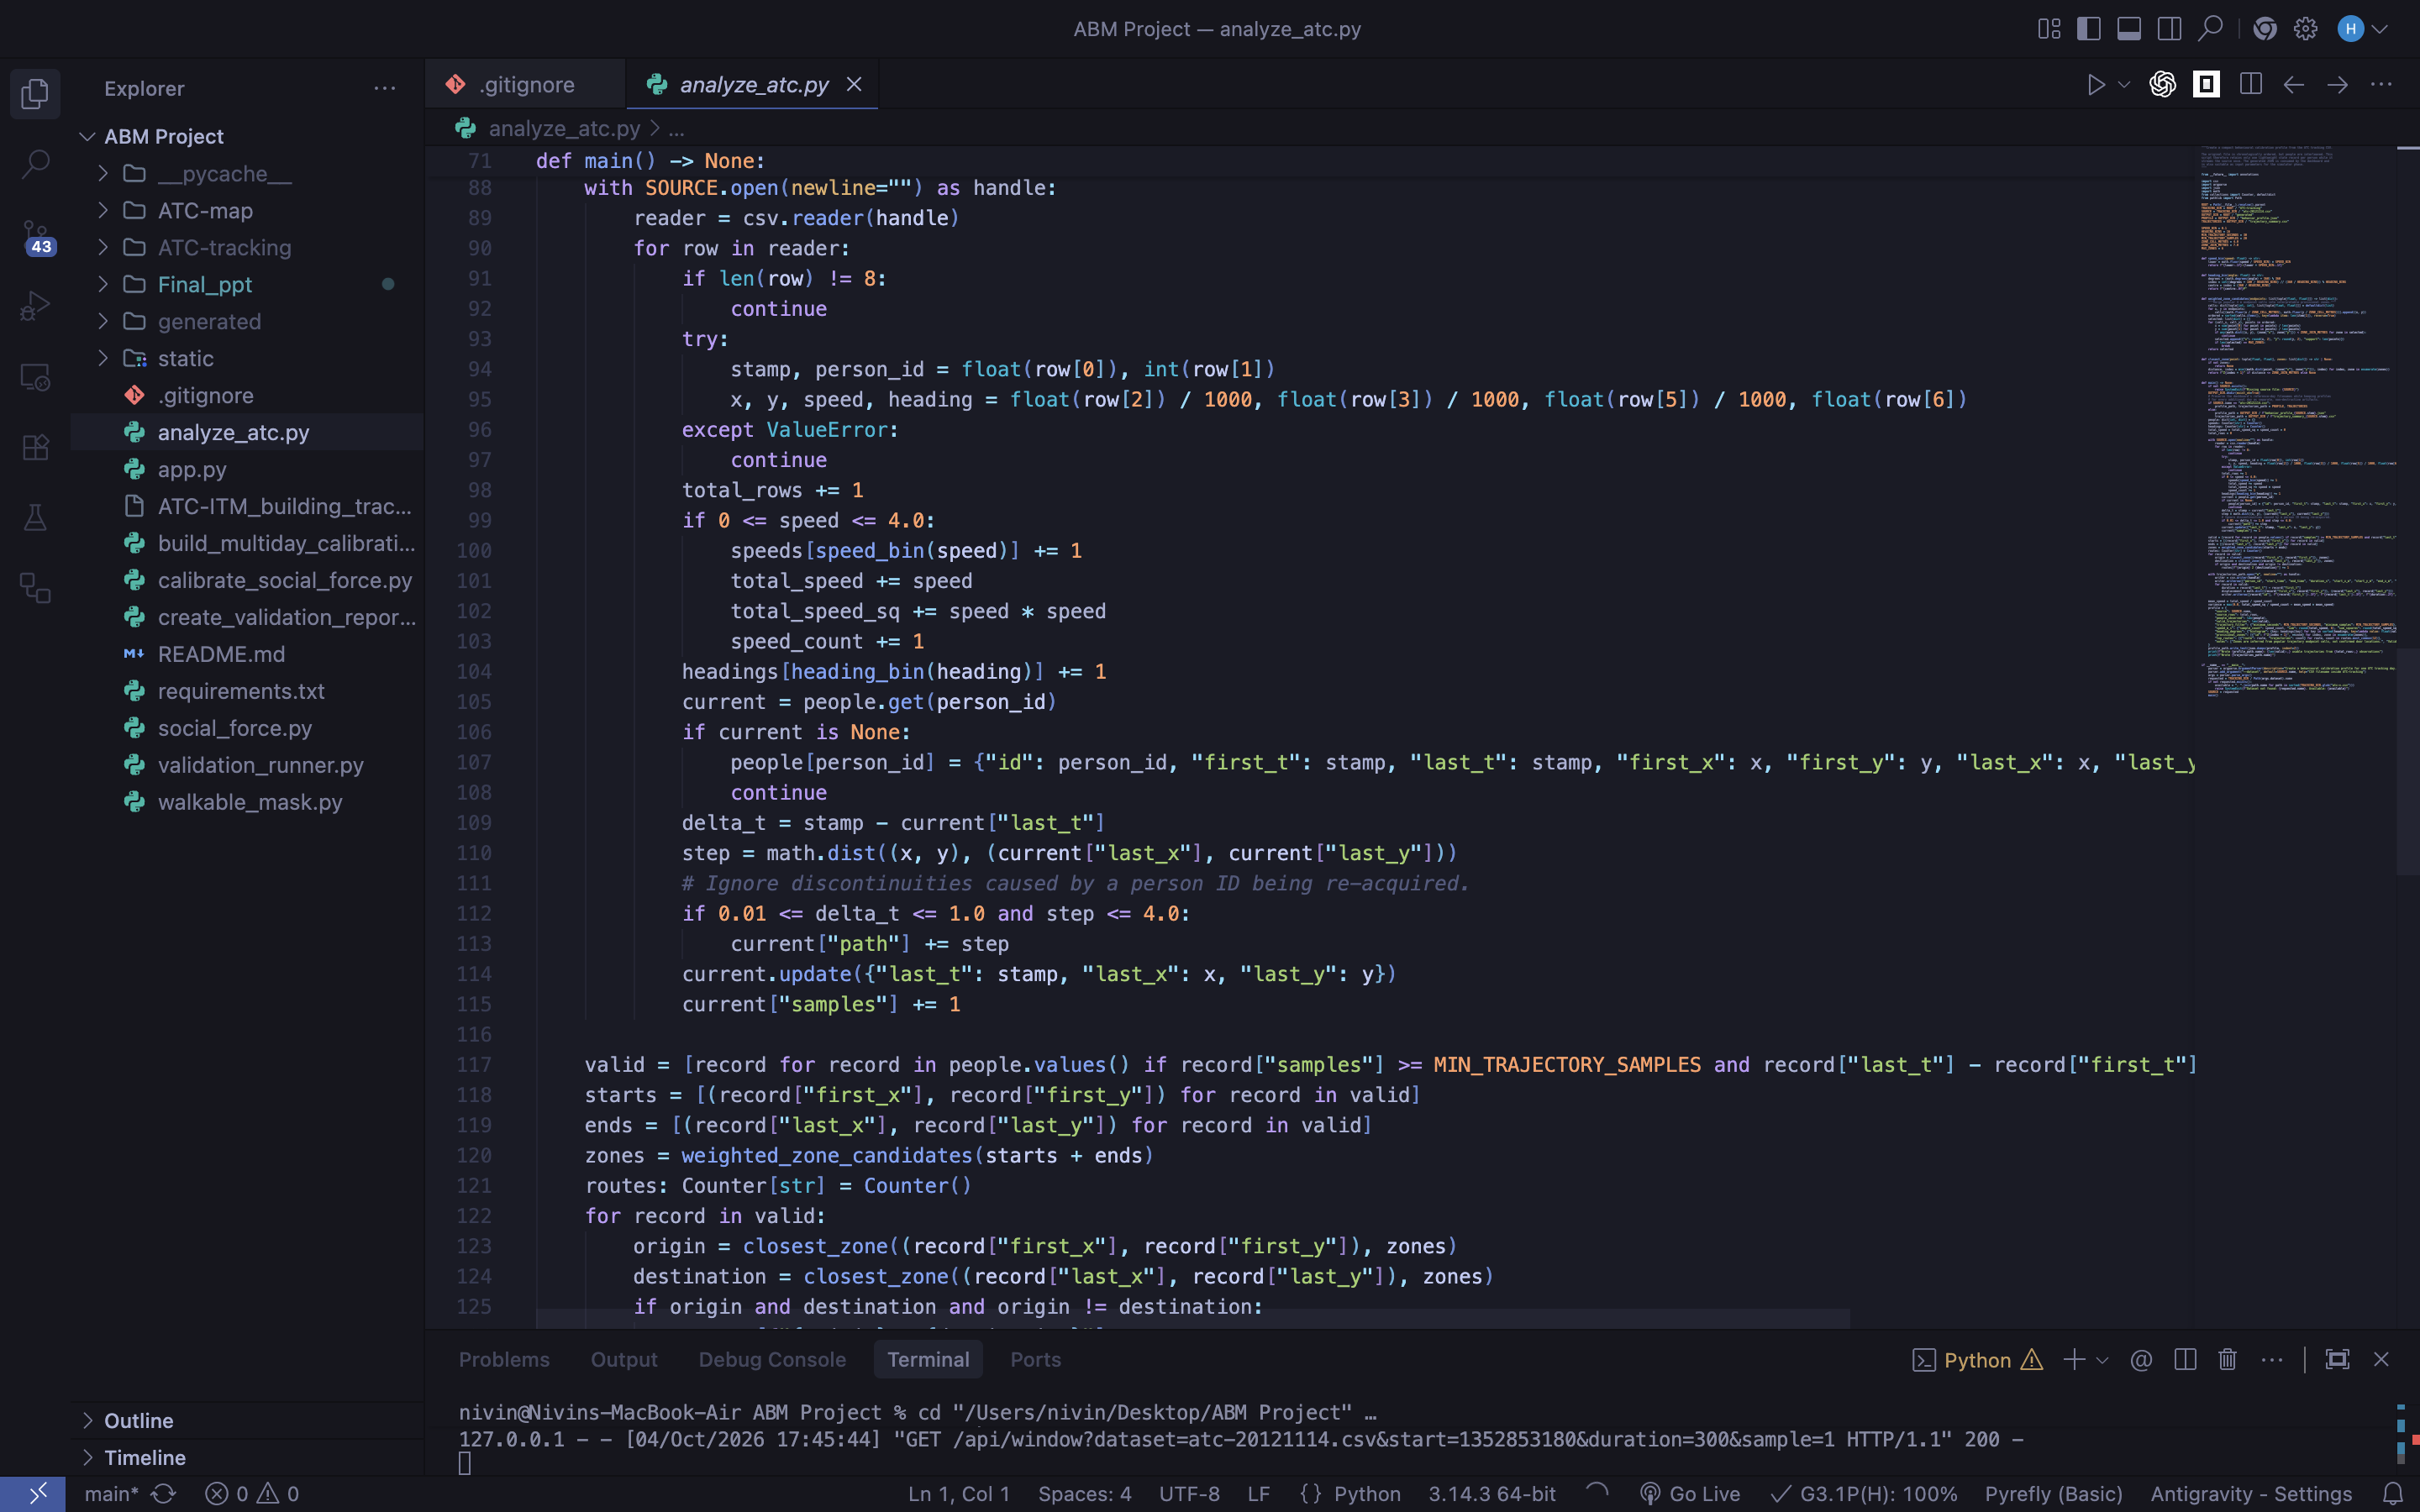
\includegraphics[trim=250bp 230bp 100bp 80bp,clip,width=0.99\textwidth,height=0.82\textheight,keepaspectratio]{code_track_cleaning.png}
\end{frame}

% 18
\begin{frame}\frametitle{Code Implementation: Social Force Model}
\centering
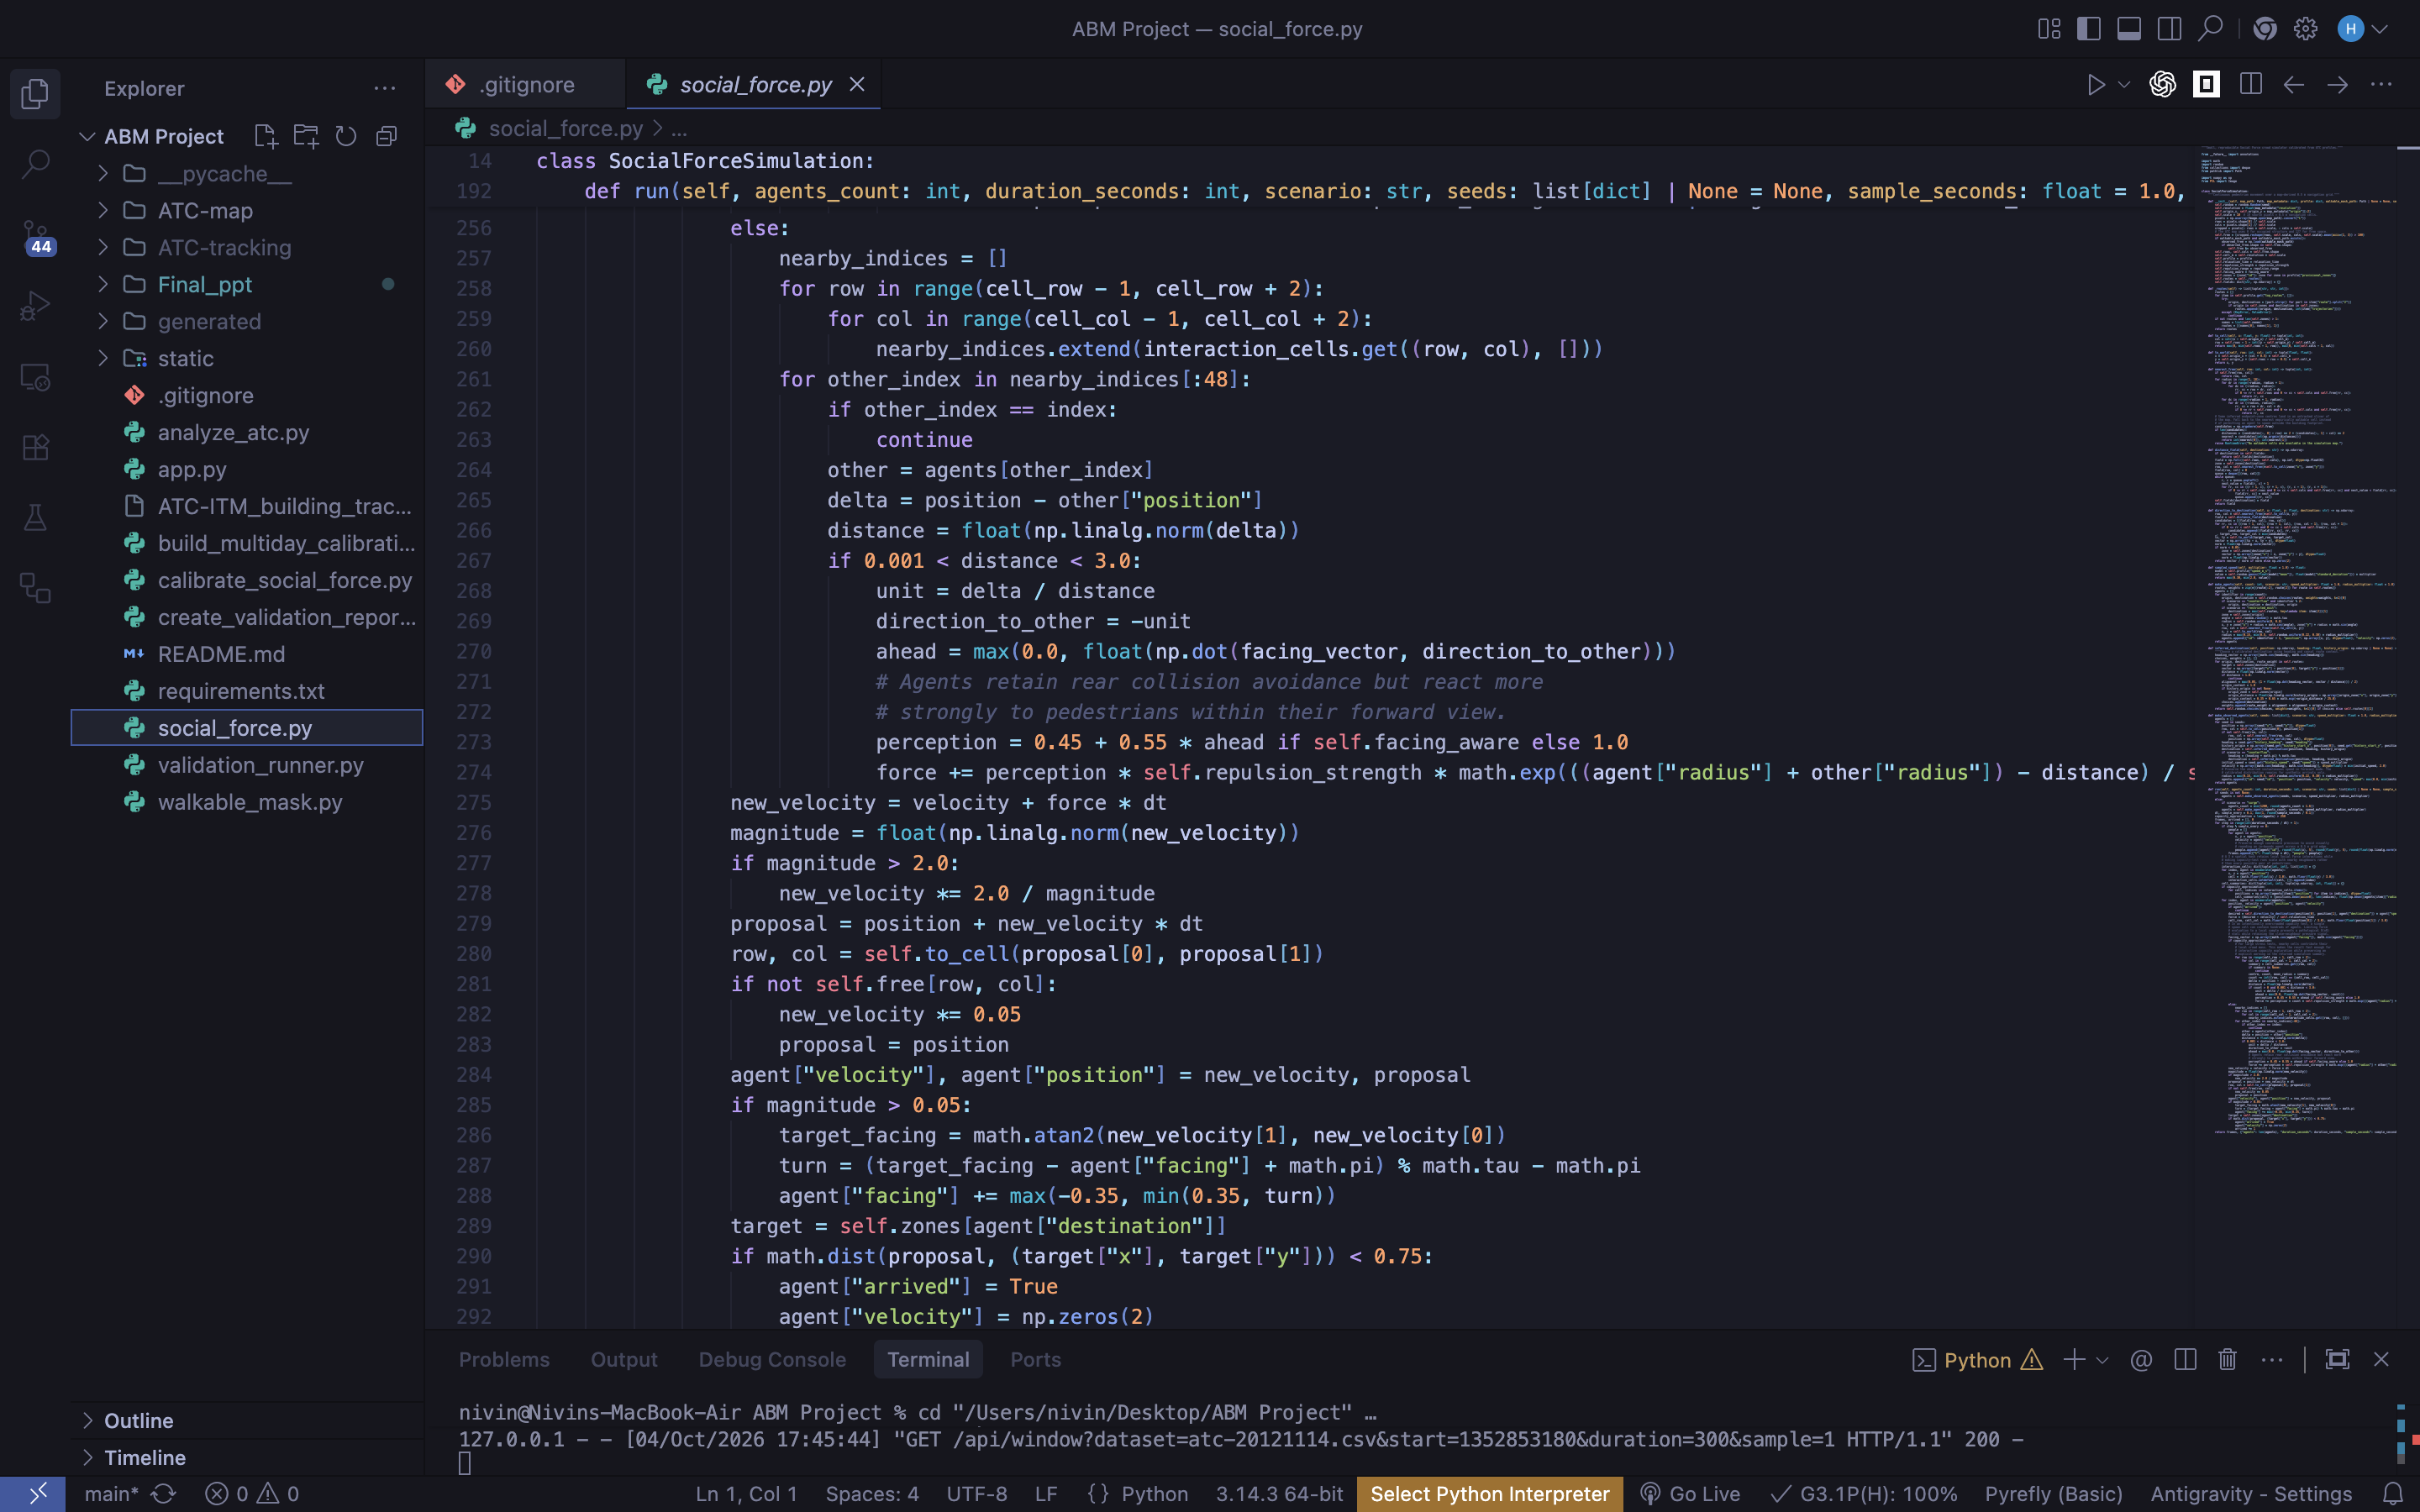
\includegraphics[trim=250bp 90bp 100bp 140bp,clip,width=0.99\textwidth,height=0.82\textheight,keepaspectratio]{code_social_force.png}
\end{frame}

% 19
\begin{frame}\frametitle{Code Implementation: Forecast Evaluation}
\centering
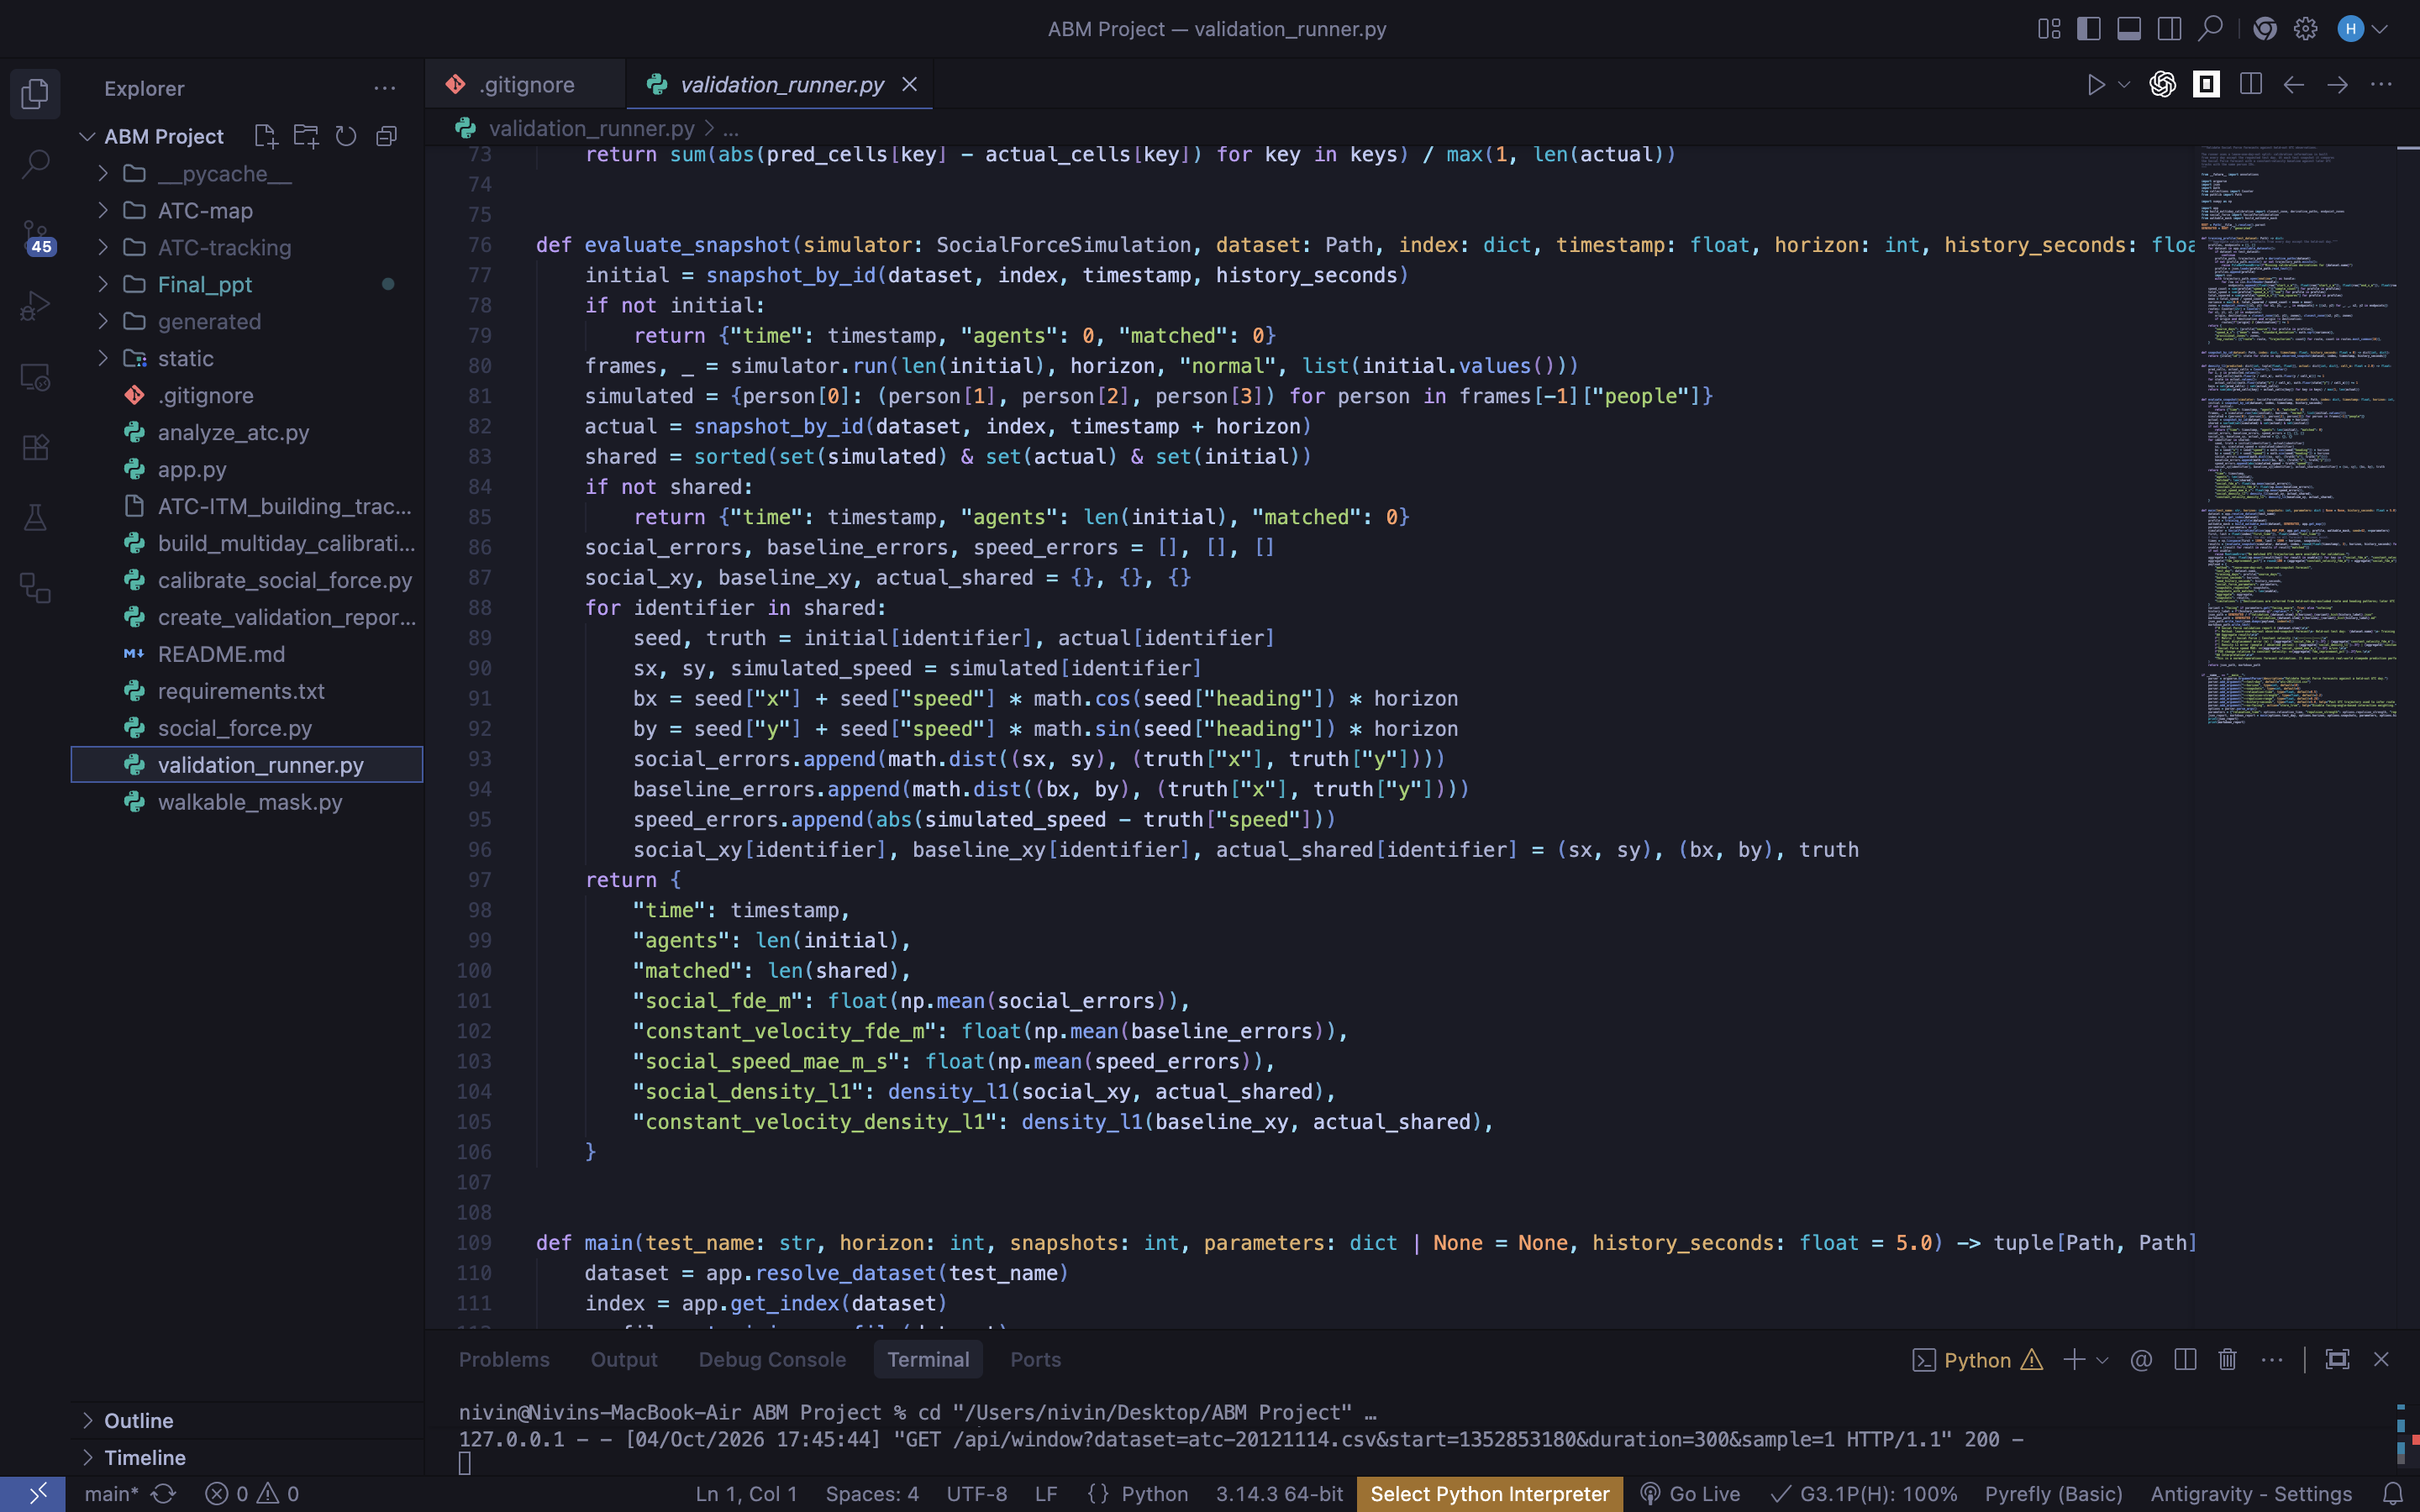
\includegraphics[trim=250bp 250bp 100bp 80bp,clip,width=0.99\textwidth,height=0.82\textheight,keepaspectratio]{code_evaluation.png}
\end{frame}

% 9 Challenges Faced
\section{Challenges Faced}
% 20
\begin{frame}\frametitle{Challenges Faced}
\begin{itemize}
\item \textbf{Large source files:} streaming reads and minute-level indexes support practical replay.
\item \textbf{Map ambiguity:} the ROS map includes broad unknown/free areas; a trajectory-derived walkable mask constrains agents.
\item \textbf{Uncertain destinations:} route intent is inferred from short history, heading, and other-day route frequencies.
\item \textbf{Limited emergency evidence:} calibration and test data describe ordinary shopping-centre flow, not crowd-crush events.
\end{itemize}
\begin{alertblock}{Main limitation}
The current metrics support short-horizon normal-flow forecasting only. They do not establish a stampede warning capability.
\end{alertblock}
\end{frame}

% 10 Future Scope
\section{Future Scope}
% 21
\begin{frame}\frametitle{Future Scope}
\begin{enumerate}
\item Integrate calibrated computer vision to turn video observations into map-aligned tracks.
\item Expand evaluation to more dates, venues, crowd densities, and independent datasets.
\item Calibrate and validate dense-flow and emergency behaviour with scenario evidence and expert-defined measures.
\item Compare exit, route, and staffing interventions using evacuation time, peak density, and uncertainty.
\end{enumerate}
\begin{block}{Long-term direction}
Develop the simulator as a decision-support tool that tests safety scenarios; treat its forecasts as model-based estimates, not guaranteed predictions.
\end{block}
\end{frame}

% 11 References
\section{Reference}
% 22
\begin{frame}\frametitle{References}
\small
{\scriptsize
\begin{enumerate}
\setlength{\itemsep}{0.04cm}
\item ATR Interaction Science Laboratories. \emph{ATC shopping-centre tracking dataset and occupancy map}.\\[-1pt]
\url{https://dil.atr.jp/ISL/crest2010_HRI/ATC_dataset/}
\item Br\v{s}\v{c}i\'c, D., Kanda, T., Ikeda, T., and Miyashita, T. (2013). Person position and body direction tracking in large public spaces using 3-D range sensors. \emph{IEEE Transactions on Human-Machine Systems}, 43(6), 522--534.
\item Khan, S. and Deng, Z. (2024). Agent-based crowd simulation: an in-depth survey of determining factors for heterogeneous behaviour. \emph{The Visual Computer}, 40, 4993--5004.\\[-1pt]
\url{https://doi.org/10.1007/s00371-024-03503-2}
\item Makinoshima, F. and Oishi, Y. (2022). Crowd flow forecasting via agent-based simulations with sequential latent parameter estimation from aggregate observation. \emph{Scientific Reports}, 12, 11168.\\[-1pt]
\url{https://doi.org/10.1038/s41598-022-14646-4}
\item Alidmat, O. et al. (2025). Simulation of crowd evacuation in asymmetrical exit layout based on improved dynamic parameters model. \emph{IEEE Access}, 13, 7512--7525.\\
\url{https://doi.org/10.1109/ACCESS.2024.3420068}
\item Helbing, D. and Moln\'ar, P. (1995). Social force model for pedestrian dynamics. \emph{Physical Review E}, 51, 4282--4286.\\
\url{https://doi.org/10.1103/PhysRevE.51.4282}
\end{enumerate}
}
\note{Literature review source: Main_lit_review (3).pdf. Dataset and project details were checked against the supplied ATC files and local implementation.}
\end{frame}

\end{document}
